% Copyright (c) 2015 William Bevington, Callum O'Brien and Alex Pace

% Permission is granted to copy, distribute and/or modify this document
% under the terms of the GNU Free Documentation License, Version 1.3
% or any later version published by the Free Software Foundation;
% with no Invariant Sections, no Front-Cover Texts, and no Back-Cover Texts.

\documentclass{article}

\usepackage{amsmath}
\usepackage{amssymb}
\usepackage{geometry}
\usepackage{tikz}

\title{C4}
\author{William Bevington \and Callum O'Brien \and Alex Pace}

\newcommand{\C}{\textit{const.}}
\newcommand{\dx}{\:\textrm{d}x}

\begin{document}

\maketitle
\tableofcontents
\newpage

\section{Parametric Curves}

Parametric curves occur when \(x\) and \(y\) are defined in terms of a parameter, a parameter being a value that is the same in both the functions for \(x\) and for \(y\). In a parametric curve \(C\) with parameter \(t\);

\[C:x=f(t),y=g(t)\]

\noindent One differentiates a parametric eqution using the chain rule. If we were to differentiate \(y\) with respect to \(x\) by the chain rule, we would find

\[\frac{\textrm{d}y}{\textrm{d}x}=\frac{\textrm{d}y}{\textrm{d}t}\frac{\textrm{d}t}{\textrm{d}x}=\frac{f'(t)}{g'(t)}\]

\noindent Integration of parametric curves is done by integrating with respect to \(t\). If one has to integrate with respect to something else, one can tranform it hence;

\[\int_{f(t)=a}^{b}g(t)\textrm{d}f(t)=\int_{t=f^{-1}(a)}^{b}g(t)f'(t)\textrm{d}t\]

\noindent This is then isomorphic to integration of non-parametric curves.

\section{Implicit Differentiation}

\[\frac{\textrm{d}}{\textrm{d}x}xy=\frac{\textrm{d}y}{\textrm{d}x}x+y\]
\[\frac{\textrm{d}}{\textrm{d}x}y^n=\frac{\textrm{d}y}{\textrm{d}x}ny^{n-1}\]

\section{Forming Differential Equations}

Differential equations describe scenarios in which;

\[\frac{\partial y}{\partial x}\propto y\]

\noindent Newton's law of cooling states that the rate of loss of temperature $-\frac{\partial\theta}{\partial t}$ is proportional to the the difference between the temperature $\theta$ of the body and the temperature $\theta_0$ of its surroundings;

\[\frac{\partial\theta}{\partial t}= -k (\theta - \theta_0)\]

\section{Integrating using Trigonometric Identites}

\subsection{Examples}

\[\int \tan^2 x \dx = \int \left(\sec^2 x - 1\right) \dx = \tan x - x + \C\]

\[\int \sin^2 x \dx = \frac{1}{2} \int \left[1 - \cos\left(2x\right)\right] \dx = \frac{1}{2} x - \frac{1}{4} \sin\left(2x\right) + \C\]

\[\int \sin\left(3x\right) \cos\left(3x\right) = \frac{1}{2} \int \sin\left(6x\right) \dx = -\frac{1}{12} \cos\left(6x\right) + \C \]

\section{Volumes of Revolution}

\begin{center}
    
    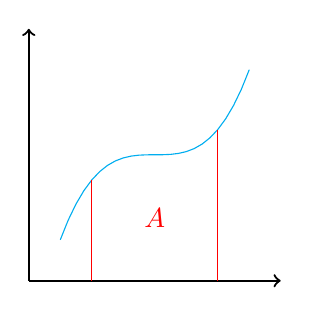
\begin{tikzpicture}[scale=0.4]
        
        \draw[->, thick] (0,0) -- (8,0);
        \draw[->, thick] (0,0) -- (0,8);
        
        \draw[cyan, domain=1:7] plot (\x, {0.1*(\x-4)*(\x-4)*(\x-4)+4});
        
        \draw[red] (2,0) -- (2,3.2);
        \draw[red] (6,0) -- (6,4.8);
        
        \node[red] at (4,2) {\(A\)};
    
    \end{tikzpicture} \hspace{40pt} 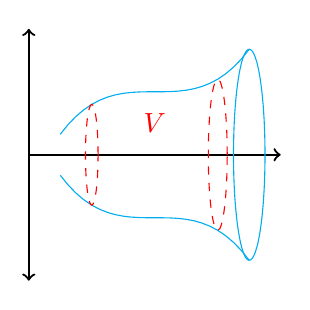
\begin{tikzpicture}[xscale=0.4,yscale=0.2]
        
        \draw[->, thick] (0,0) -- (8,0);
        \draw[<->, thick] (0,-8) -- (0,8);
        
        \draw[cyan, domain=1:7] plot (\x, {0.1*(\x-4)*(\x-4)*(\x-4)+4});
        \draw[cyan, domain=1:7] plot (\x, {-0.1*(\x-4)*(\x-4)*(\x-4)-4});
        
        \draw[cyan] (7,0)  ellipse (0.5 and 6.7);
        
        \draw[red, dashed] (2,0) ellipse (0.2 and 3.2);
        \draw[red, dashed] (6,0) ellipse (0.3 and 4.8);
        
        \node[red] at (4,2) {\(V\)};
    
    \end{tikzpicture}

\end{center}

\noindent To calculate the volume if \(y=f(x)\) has been revolved around the x-axis, we can model the volume of that as a cylinder with radius that varies with \(y\). \\
\(\pi y^2\) would be the `surface area' of a given cross section. Therefore, the following would give you the volume between a point \(a\) and \(b\):

\[\int^b_a\pi y^2dx \;\;\rightarrow\;\; \pi\int^b_ay^2dx\]

\end{document}
